\chapter{Differentiable FSI Simulator and Shape \& Gait Optimization} \label{chapControl}

\section{Differentiable Fluid-Robot Multiphysics Simulation}
\label{sec:fsi_simulator}

This section summarizes a collaborative line of work on differentiable simulation for strongly coupled fluid--robot interaction, which serves as the simulation foundation for the optimization and control studies developed later in this chapter. In swimming robots, body motion and surrounding flow evolve in a tightly coupled manner: the robot deforms the fluid boundary conditions, while the fluid stress distribution in turn determines the forces and moments acting on the robot. For this reason, accurately modeling robotic swimming requires a simulator that captures the coupled evolution of articulated body dynamics and incompressible flow, rather than treating the two as only loosely connected subsystems.

To address this, we adopt a unified variational formulation of fluid--robot multiphysics. The articulated robot and the surrounding incompressible Newtonian fluid are described within a common least-action framework, from which the coupled governing equations are derived consistently. The resulting continuous-time formulation is then discretized using variational time integration, leading to an implicit and differentiable simulator suitable for gait optimization and downstream control design. This overall problem setting is illustrated in Fig.~\ref{fig:thesis_fsi_problem_setup}, where the fluid domain, the immersed robot body, and the fluid--robot interface are defined explicitly. The corresponding unified modeling perspective is further summarized in Fig.~\ref{fig:thesis_fsi_framework}. These figures are adapted from the collaborative simulator paper and included here because they provide the methodological foundation for the remainder of this chapter.

\begin{figure}[t]
    \centering
    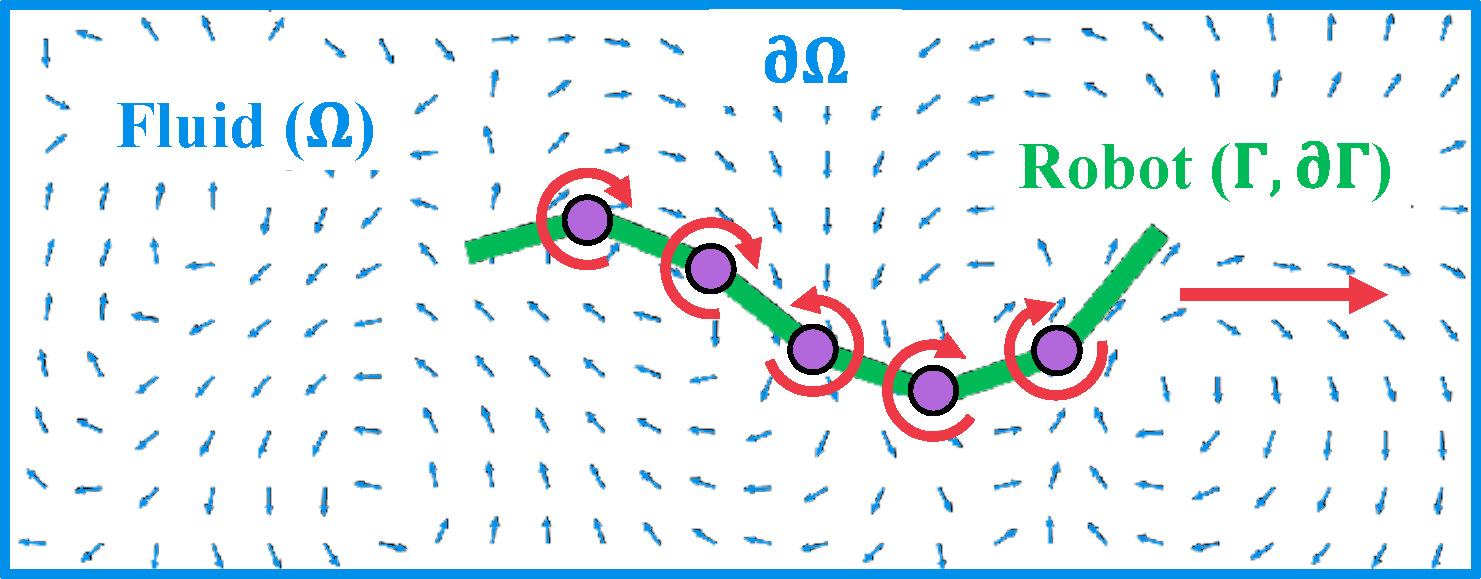
\includegraphics[width=0.78\linewidth]{figs/fsi/figure2_problem_setup.pdf}
    \caption{Problem setup for strongly coupled fluid--robot interaction. The robot body is immersed in an incompressible fluid domain $\Omega$, with dynamics coupled through the no-slip condition at the fluid--robot interface $\Gamma$. This figure is included to define the geometric setting used throughout the simulator derivation.}
    \label{fig:thesis_fsi_problem_setup}
\end{figure}

\begin{figure}[t]
    \centering
    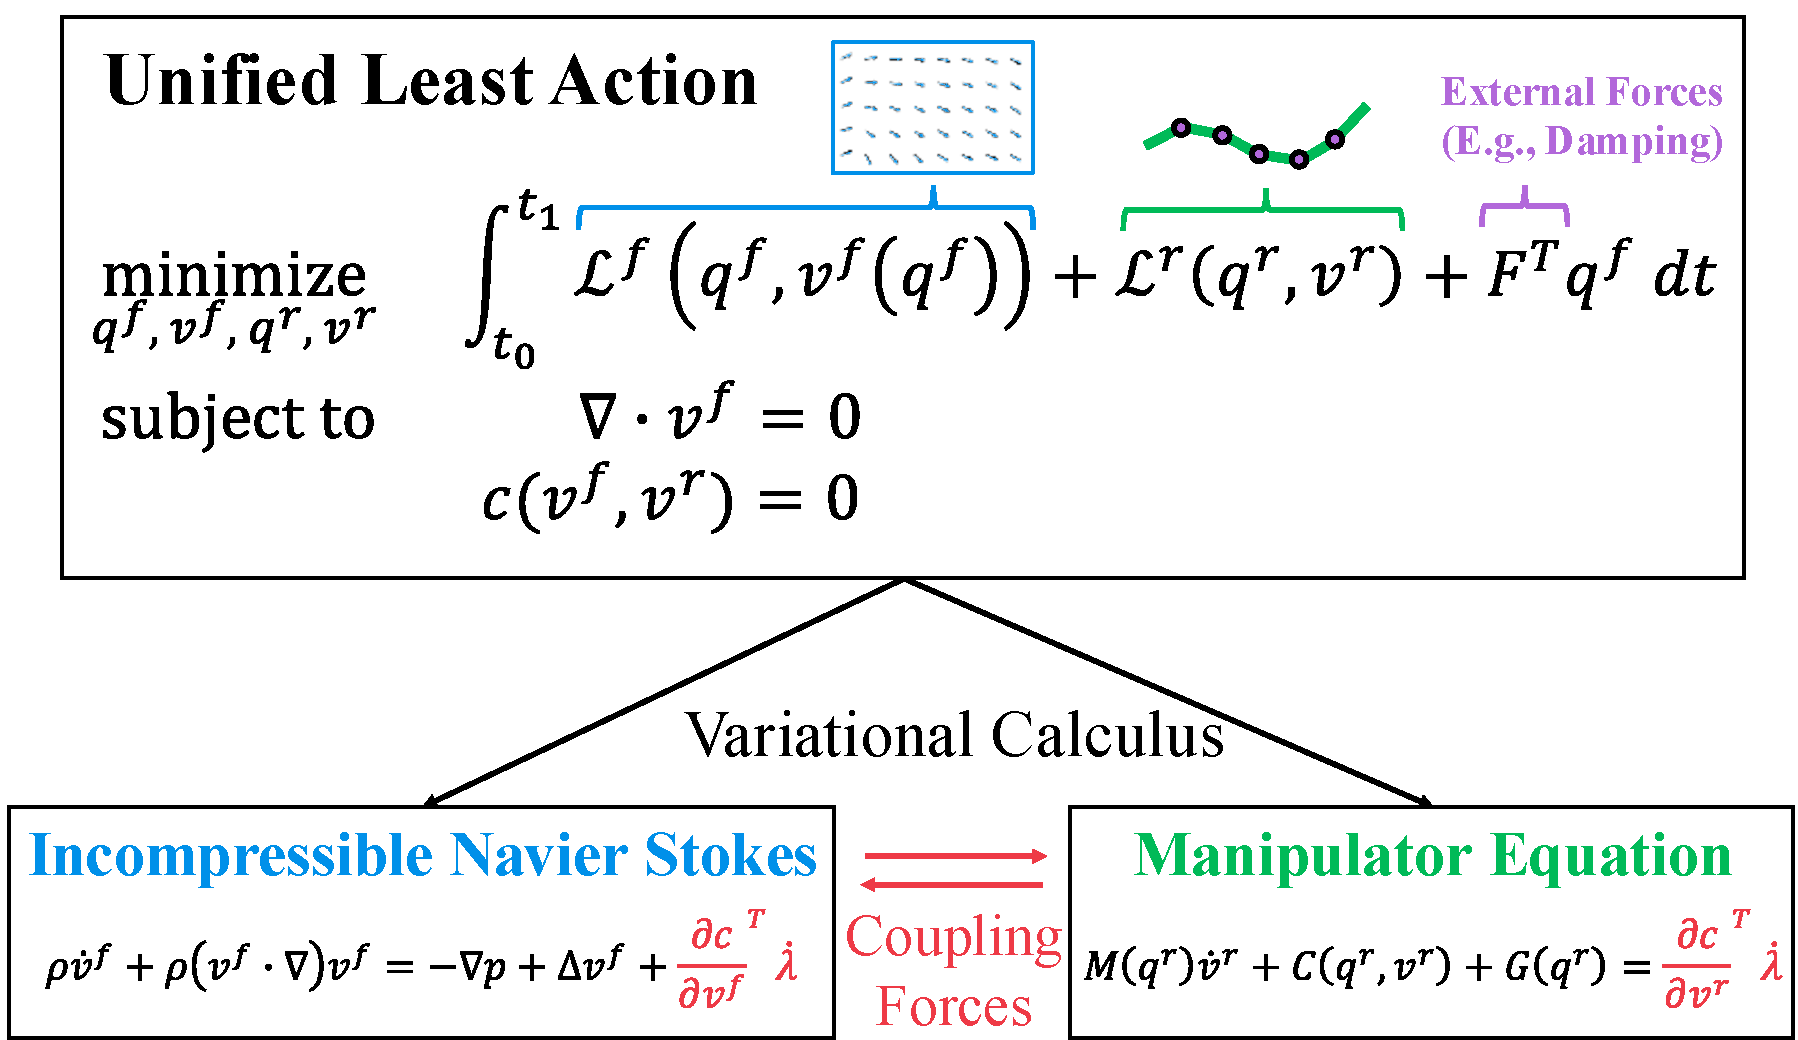
\includegraphics[width=0.82\linewidth]{figs/fsi/figure3_physics_comparison.pdf}
    \caption{Conceptual overview of the unified fluid--robot simulator. Rather than solving the robot and fluid as two separate systems and coupling them afterward, the combined action is formulated and discretized directly, leading to a strongly coupled implicit simulation scheme.}
    \label{fig:thesis_fsi_framework}
\end{figure}

\subsection{Motivation and Overview}

Many existing multiphysics simulators in robotics are built by coupling separate engines for rigid-body dynamics and fluid dynamics. While such a modular strategy is often practical, it can become inaccurate when interaction is strong, especially in swimming, where propulsion itself emerges from unsteady vortex-body coupling. In these settings, the robot state and the fluid state should not be viewed as evolving independently. Instead, they should be treated as parts of a single coupled dynamical system.

The simulator summarized in this section was developed with this perspective in mind. Starting from a unified least-action principle, the fluid and robot equations are derived together as one constrained optimization problem. The formulation is then discretized through discrete variational mechanics, yielding an implicit update rule for both the fluid velocity field and the robot state. Importantly, because the simulator step is defined implicitly, derivatives of the dynamics can be obtained through the implicit function theorem, enabling gradient-based gait optimization.

\subsection{Unified Fluid-Robot Formulation}

Let $\Omega$ denote the fluid domain and $\Gamma$ denote the robot body immersed in the fluid. The robot configuration and velocity are denoted by $q^r$ and $v^r$, while the fluid particle configuration and velocity field are denoted by $q^f$ and $v^f$. The coupled dynamics are posed through the following constrained least-action problem:
\begin{equation}
\begin{aligned}
\min_{q^r,q^f,v^r,v^f}\quad & \int_{t_0}^{t_f} L^f(q^f,v^f) + L^r(q^r,v^r) + F(t)^T q^f \, dt \\
\text{s.t.}\quad 
& \dot{q}^f - v^f(q^f) = 0, \\
& \nabla \cdot v^f = 0, \\
& v^f - v_{bc} = 0 \quad \text{on } \partial \Omega, \\
& \dot{q}^r - v^r = 0, \\
& c_5(q^r) = 0, \\
& v^f - {}^b v^r = 0 \quad \text{on } \Gamma .
\end{aligned}
\label{eq:thesis_fsi_unified_opt}
\end{equation}

Here, the first constraint defines fluid kinematics, the second enforces incompressibility, the third imposes fluid boundary conditions, the fourth is the robot kinematic relation, the fifth captures robot configuration constraints such as joints, and the last is the no-slip condition at the fluid--robot interface. As emphasized in the original simulator work, this no-slip constraint is the key source of multiphysics coupling between the robot and the surrounding flow.

The fluid and robot Lagrangians are written as
\begin{equation}
L^f(q^f,v^f) = \int_{\Omega} \frac{1}{2}\rho (v^f)^T v^f - \rho g^T q^f \, dV,
\label{eq:thesis_fluid_lagrangian}
\end{equation}
\begin{equation}
L^r(q^r,v^r) = \frac{1}{2}(v^r)^T M^r v^r - M^r g^T q^r,
\label{eq:thesis_robot_lagrangian}
\end{equation}
where $\rho$ is the fluid density, $M^r$ is the robot mass matrix, and $g$ is gravity. Viscous effects are incorporated through the non-conservative virtual-work term
\begin{equation}
F(t) = \int_{\Omega} \mu \Delta v^f \, dV,
\label{eq:thesis_viscous_force}
\end{equation}
with $\mu$ the dynamic viscosity.

Introducing Lagrange multipliers for the constraints gives the combined action
\begin{equation}
S = \int_{t_0}^{t_f} L^f + L^r + F^T q^f + \sum_i \lambda_i c_i \, dt .
\label{eq:thesis_combined_action}
\end{equation}
Taking first-order optimality conditions yields the coupled fluid--robot equations. The fluid side recovers the incompressible Navier--Stokes equations with additional constraint forces associated with the outer boundary and the fluid--robot interface:
\begin{equation}
\rho \left(\dot{v}^f + (v^f \cdot \nabla) v^f \right)
= - \nabla p + \mu \nabla^2 v^f - \rho g
- \left(\frac{\partial c_3}{\partial v^f}\right)^T \dot{\lambda}_3
- \left(\frac{\partial c_6}{\partial v^f}\right)^T \dot{\lambda}_6,
\label{eq:thesis_ns_coupled}
\end{equation}
together with
\begin{equation}
\nabla \cdot v^f = 0.
\label{eq:thesis_incompressibility}
\end{equation}

The robot side follows the manipulator dynamics augmented by the reaction force arising from the no-slip constraint:
\begin{equation}
M^r \dot{v}^r + M^r g
=
\left(\frac{\partial c_5}{\partial q^r}\right)^T \lambda_5
-
\left(\frac{\partial c_6}{\partial v^r}\right)^T \dot{\lambda}_6,
\label{eq:thesis_robot_coupled}
\end{equation}
with
\begin{equation}
\dot{q}^r = v^r.
\label{eq:thesis_robot_kinematics}
\end{equation}

This formulation is important for the dissertation not only because it provides a physically grounded model of swimming, but also because it shows that fluid dynamics and articulated robot dynamics can be derived from a single constrained variational principle rather than stitched together heuristically afterward. This viewpoint is central to the optimization-based treatment adopted later in this chapter.

\subsection{Variational Time Discretization}

To simulate the coupled system stably, the continuous action is discretized directly using discrete variational mechanics. Compared with explicitly integrating the resulting differential equations, this strategy tends to provide better numerical stability and more consistent constraint treatment in strongly coupled systems.

A midpoint discrete Lagrangian is introduced as
\begin{equation}
L_d(q_k,q_{k+1})
=
h\,L\!\left(
\frac{q_k+q_{k+1}}{2},
\frac{q_{k+1}-q_k}{h}
\right),
\label{eq:thesis_midpoint_dl}
\end{equation}
where $h$ is the simulation time step. A practical complication is that the robot is naturally represented by configurations, while the fluid is more naturally represented by a velocity field. Following the simulator formulation, the discrete state is therefore organized around robot configurations and midpoint fluid velocities.

The fluid domain is spatially discretized using a finite-volume scheme, producing discrete operators for inertia, pressure, convection, and viscosity. In discrete form, the fluid Lagrangian becomes
\begin{equation}
L^f(q^f,v^f) = \frac{1}{2}(v^f)^T M^f v^f - (M^f g)^T q^f,
\label{eq:thesis_discrete_fluid_lagrangian}
\end{equation}
where $M^f$ is the discrete fluid mass matrix.

Applying the discrete first-order conditions leads to an implicit update rule for the coupled system. The robot configuration update is
\begin{equation}
q^r_{k+1} = q^r_k + h \bar{v}^r_{k+1},
\label{eq:thesis_robot_update}
\end{equation}
and the robot velocity equation takes the form
\begin{equation}
\frac{1}{2} M^r \bar{v}^r_{k+1}
- h \left( \frac{\partial c_5}{\partial q^r_k} \right)^T \lambda_{5,k}
- h \left( \frac{\partial c_6}{\partial \bar{v}^r_k} \right)^T \lambda_{6,k}
=
\frac{1}{2} M^r \bar{v}^r_k - h M^r g .
\label{eq:thesis_robot_variational}
\end{equation}

Similarly, the fluid update is
\begin{equation}
\begin{aligned}
\frac{1}{2}(M^f - \mu h L)\bar{v}^f_{k+1}
- \frac{h}{2} N(\bar{v}^f_{k+1})
+ G p_k
+ B \lambda_{3,k}
- h \left(\frac{\partial c_6}{\partial \bar{v}^f_k}\right)^T \lambda_{6,k} \\
=
\frac{1}{2}(M^f + \mu h L)\bar{v}^f_k
+ \frac{h}{2} N(\bar{v}^f_k)
- h M^f g ,
\end{aligned}
\label{eq:thesis_fluid_variational}
\end{equation}
subject to the discrete incompressibility, boundary, no-slip, and robot-constraint conditions:
\begin{align}
G^T \bar{v}^f_{k+1} &= 0, \label{eq:thesis_disc_incompressibility} \\
B\bar{v}^f_{k+1} - v_{bc} &= 0, \label{eq:thesis_disc_bc} \\
E\bar{v}^f_{k+1} - {}^b\bar{v}^r(\bar{v}^r_{k+1}) &= 0, \label{eq:thesis_disc_noslip} \\
c_5(q^r_{k+1}) &= 0. \label{eq:thesis_disc_robotconstraint}
\end{align}

These equations are solved jointly at each time step, typically with Newton iterations, yielding a stable implicit integrator for the coupled fluid--robot dynamics. In the context of this dissertation, the main importance of this step is that the simulator is not merely a forward physics model; it is a structured computational object whose implicit solve can later be differentiated and used for optimization.

\subsection{Integral-Form No-Slip Coupling}

One practical challenge in immersed-boundary-style coupling is that the standard no-slip constraint is often enforced only at a finite set of discrete boundary nodes:
\begin{equation}
Ev^f - {}^b v^r = 0.
\label{eq:thesis_classic_ibm}
\end{equation}
Although simple, this pointwise treatment can become problematic in robotic multibody systems. If the boundary discretization is too sparse, fluid leakage may appear between constraint points. Conversely, when multiple body segments come close to one another, the resulting constraints may become redundant or ill-conditioned.

To alleviate these issues, the simulator extends the classical immersed boundary method by adopting an integral, or weak-form, treatment of the no-slip relation. Instead of enforcing equality only at isolated nodes, the coupling is integrated over the body boundary:
\begin{equation}
\oint_{\Gamma} \int_{\Omega}
v^f \, \delta(q^f - {}^b q^r(q^r)) \, dV\, dS
=
\oint_{\Gamma} {}^b v^r(q^r,v^r)\, dS .
\label{eq:thesis_weak_ibm_cont}
\end{equation}

After piecewise-linear discretization along the boundary, this leads to an integrated convolution operator $\bar{E}$ and the discrete weak-form constraint
\begin{equation}
\bar{E}v^f - {}^b v^r(v^r) = 0.
\label{eq:thesis_weak_ibm_disc}
\end{equation}

This weak-form extension was one of the key methodological contributions of the original simulator work, where it was introduced specifically to make the no-slip coupling more robust and better conditioned for articulated robotic systems. Compared with directly enforcing pointwise matching at a sparse set of markers, this formulation is less sensitive to geometric discretization and more suitable for bodies with multiple closely spaced segments.

\subsection{Differentiability and Role in This Dissertation}

Because each simulator step is defined as the solution of an implicit nonlinear system, derivatives of the next state with respect to the current state and control inputs can be computed through the implicit function theorem. This makes the simulator differentiable end-to-end and allows gradients to be used for downstream optimization tasks, including gait design and trajectory refinement. The differentiable nature of the simulator was emphasized in the original work as one of its central benefits for robotic swimming and learning-based applications.

In the associated study, the simulator was validated on a bioinspired eel robot in both steady undulatory swimming and a highly dynamic C-start maneuver. In particular, the C-start task provided a useful test of whether the simulator could capture aggressive transient fluid--body interaction and whether the resulting gradients could support meaningful gait optimization. The original paper also compared these results against a smoothed-particle hydrodynamics baseline implemented in Genesis, showing that the unified formulation better matched the physical hardware for this maneuver. A representative example is shown in Fig.~\ref{fig:thesis_cstart_result}, which is included here not to fully reproduce the original experimental section, but to illustrate the level of dynamic behavior that the simulator can support and the sim-to-real relevance of the framework.

\begin{figure}[t]
    \centering
    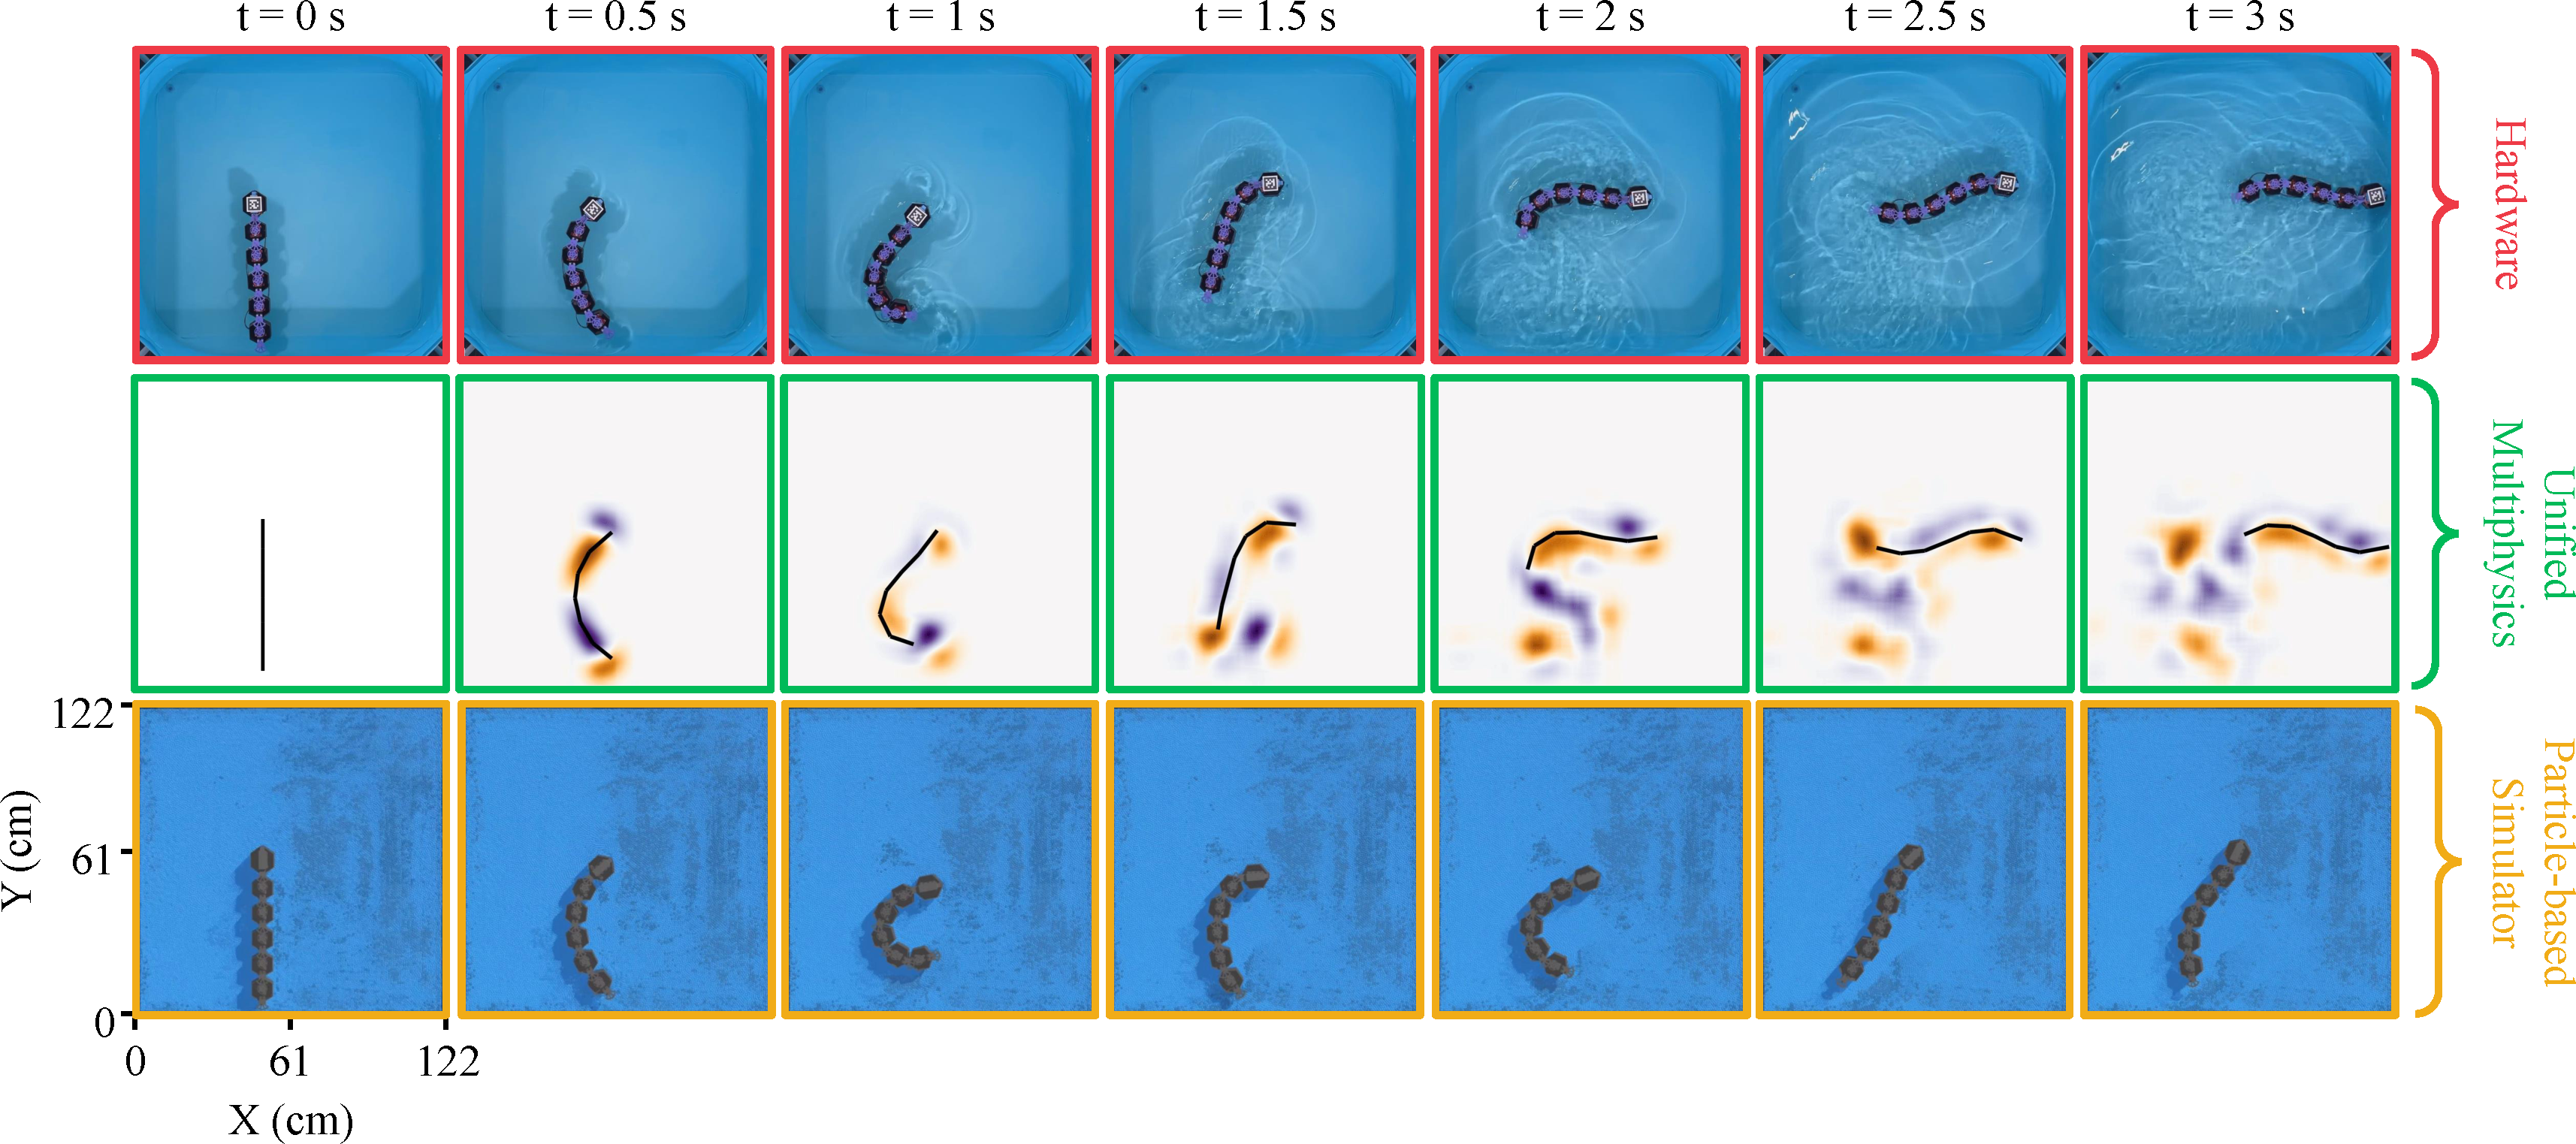
\includegraphics[width=1\linewidth]{figs/fsi/figure1_eel_c_start_optimal_timepoints.pdf}
    \caption{Representative validation result for the differentiable fluid--robot simulator on a highly dynamic C-start maneuver. The optimized gait, obtained using gradients from the simulator, transfers successfully to the physical eel robot and produces the intended turning behavior. This result illustrates the simulator's relevance for trajectory optimization and sim-to-real transfer.}
    \label{fig:thesis_cstart_result}
\end{figure}

For this dissertation, the simulator is not treated as an end in itself. Rather, it serves as a methodological foundation for the remaining sections of this chapter in two ways. First, it provides a physics-based differentiable environment for shape and gait optimization in swimming robots. Second, it establishes a principled route from fluid mechanics to optimization and feedback control, which motivates the sim-to-real transfer strategy based on iterative learning control in the next section and the feedback stabilization study under flow disturbances later in the chapter.


\subsection{Experimental Validation}
\label{sec:fsi_experimental_validation}

To evaluate the fidelity of the unified fluid--robot simulator and its usefulness for gait optimization, we validated the framework against hardware experiments on a multilink eel robot. This section summarizes the experimental setup, the forward-swimming comparison, and the C-start gait optimization results. The hardware platform and pool experiments were developed as part of this dissertation work, while the simulator implementation and baseline comparisons were carried out collaboratively.

\subsubsection{Experimental Setup}

The hardware platform is a five-link planar eel robot actuated by Dynamixel XC330 servo motors mounted on an OpenRB-150 control board. Each joint is driven by position commands generated from a parameterized gait pattern, and the resulting body motion is tracked using an overhead camera system with AprilTag fiducial markers attached to each link. The robot swims at the surface of a pool, and the recorded trajectories are post-processed using cubic spline interpolation to obtain smooth position and heading estimates for each link over time.

On the simulation side, two methods are compared against hardware:
\begin{itemize}
    \item \textbf{Unified multiphysics}: the differentiable fluid--robot simulator described in the preceding sections, which solves the coupled Navier--Stokes and articulated-body equations jointly through the variational formulation.
    \item \textbf{SPH baseline}: a smoothed-particle-hydrodynamics (SPH) based fluid coupling implemented in Genesis, which treats the fluid and robot as loosely coupled subsystems.
\end{itemize}
Both simulators receive the same joint-angle trajectories as input and produce predicted head-link configuration trajectories (position and heading) as output. Accuracy is measured by the root-mean-square error (RMSE) between simulated and hardware-recorded head-link trajectories.

\subsubsection{Forward Swimming Validation}

We first evaluate both simulators on steady undulatory forward swimming. The robot executes a sinusoidal traveling-wave gait at four joint-angle amplitudes: $10^\circ$, $20^\circ$, $30^\circ$, and $40^\circ$, with 20 trials conducted per amplitude to capture run-to-run variability.

\begin{figure}[t]
    \centering
    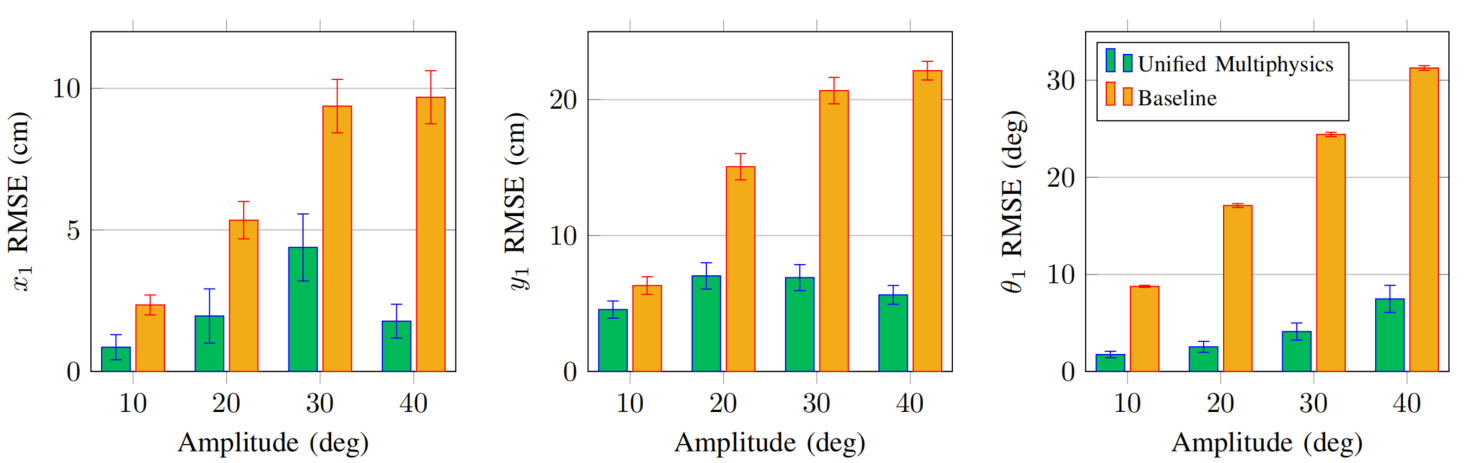
\includegraphics[width=\linewidth]{figs/fsi/Figure8xythetaerror.png}
    \caption{Average root-mean-square error (RMSE) and associated standard deviations for simulated versus hardware-validated trajectories of the head-link configuration. Results are shown for joint-angle amplitudes of $10^{\circ}$, $20^{\circ}$, $30^{\circ}$, and $40^{\circ}$ across 20 trials per amplitude. The unified fluid--robot multiphysics simulator (green) consistently outperforms the SPH baseline (orange) across all undulation amplitudes, with the improvement becoming more pronounced at higher amplitudes. At $40^{\circ}$ amplitude, error reductions reach as high as 75\% compared to the baseline, demonstrating that strongly coupled fluid--robot simulation significantly improves fidelity for robotic swimming.}
    \label{fig:forward_swimming_rmse}
\end{figure}

Fig.~\ref{fig:forward_swimming_rmse} summarizes the RMSE comparison across all amplitudes. The unified multiphysics simulator consistently outperforms the SPH baseline at every amplitude tested, and the gap widens at higher amplitudes where the fluid--body coupling is stronger. At $40^\circ$ amplitude, the unified formulation achieves up to 75\% lower RMSE than the baseline. This trend is expected: at larger amplitudes the body undergoes more aggressive deformation, generating stronger vortex--body interactions that a loosely coupled solver struggles to capture.

\begin{figure}[t]
    \centering
    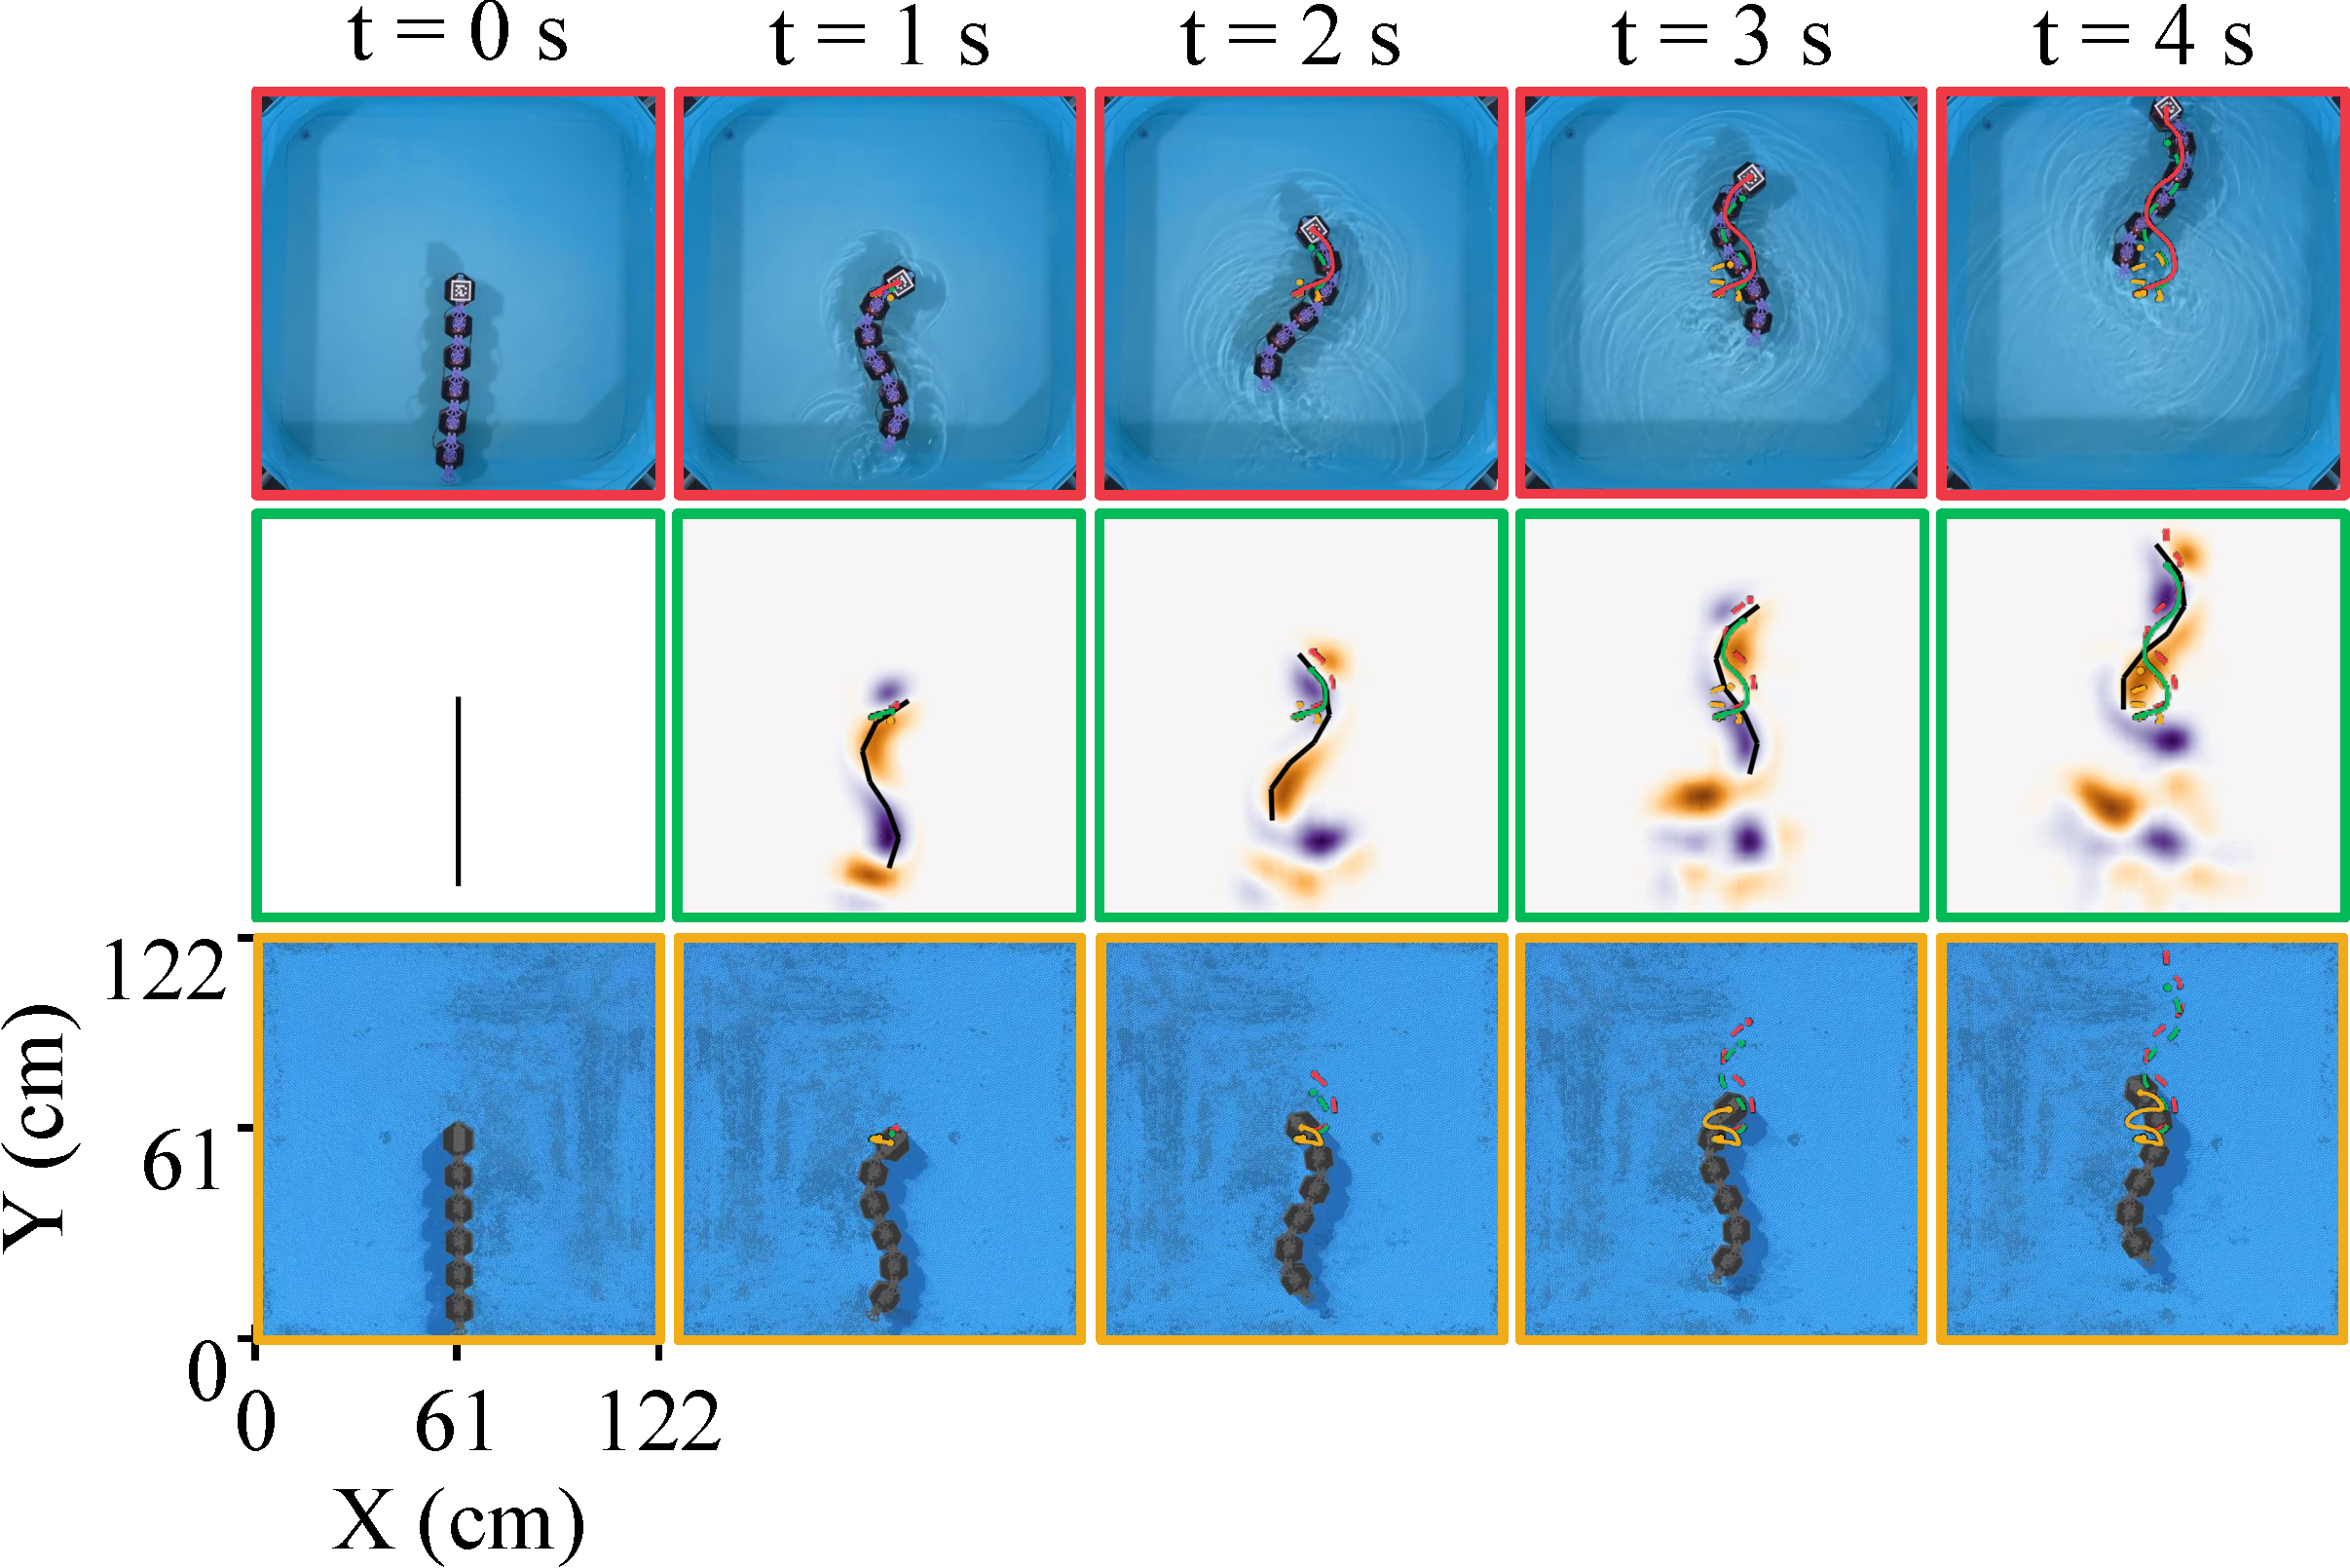
\includegraphics[width=0.8\linewidth]{figs/fsi/figure9_eel_forward_swimming_timepoints.pdf}
    \caption{Time-lapse sequences showing the multilink eel robot executing an undulating gait with a $40^\circ$ joint-angle amplitude for forward swimming. The top row (red) shows the real-world robot, the middle row (green) shows the unified multiphysics simulator, and the bottom row (orange) shows the SPH baseline. The unified method closely tracks the forward displacement observed in hardware, while the SPH baseline produces comparatively little forward progress.}
    \label{fig:thesis_forward_swimming_timelapse}
\end{figure}

A qualitative comparison at $40^\circ$ amplitude is shown in Fig.~\ref{fig:thesis_forward_swimming_timelapse}. The time-lapse sequences illustrate that the unified simulator closely reproduces the forward displacement and body shape observed in the real robot, whereas the SPH baseline substantially underestimates the swimming speed and produces a visibly different body trajectory. This qualitative difference is consistent with the quantitative RMSE results and underscores the importance of strongly coupled simulation for predicting undulatory swimming performance.

\subsubsection{C-Start Gait Optimization}

Beyond forward swimming, we also validate the simulator on a more challenging maneuver: the C-start escape turn. A C-start is a rapid, transient maneuver in which the robot bends its body into a C-shape and then straightens to achieve a large heading change in a short time. This maneuver involves highly unsteady vortex shedding and strong fluid--body interaction, making it a stringent test of simulator fidelity.

The C-start gait is parameterized by the joint-angle profiles over a fixed time horizon, and the differentiable simulator is used to optimize these profiles via gradient descent. The optimization objective is to maximize the heading change achieved during the maneuver. Both the initial (pre-optimization) and optimized gaits are then executed on the physical robot for comparison.

\begin{figure}[t]
    \centering
    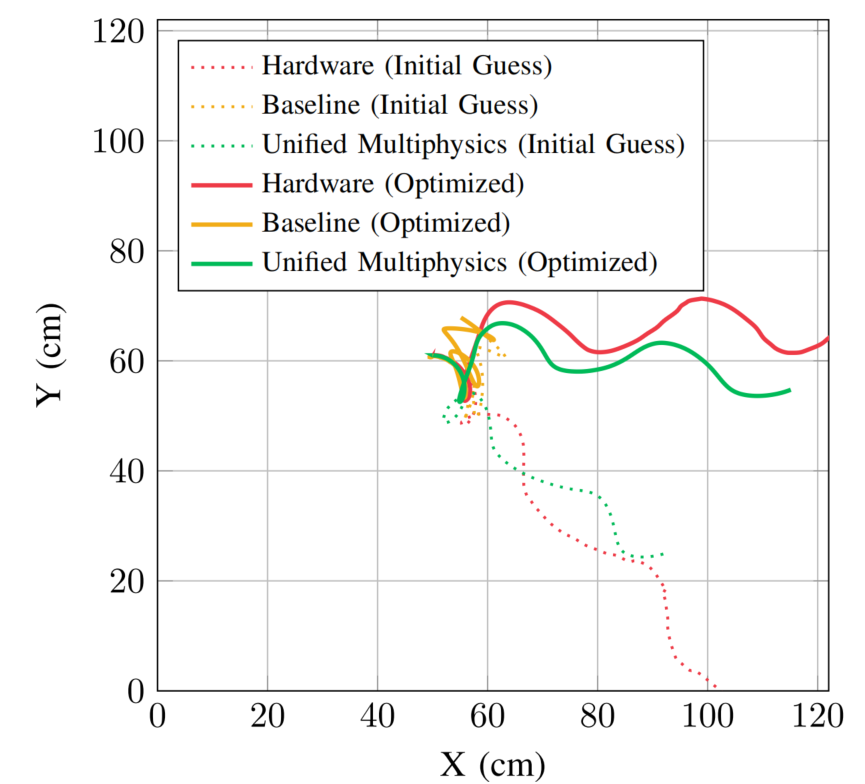
\includegraphics[width=0.7\linewidth]{figs/fsi/figure11_optimal.png}
    \caption{Head-link configuration trajectories for the multilink eel robot executing a C-start turn. Dotted lines represent trajectories generated by the initial gait prior to optimization, while solid lines correspond to those produced by the optimized gait. The unified multiphysics approach (green) achieves a heading direction close to that of hardware (red) for both cases, demonstrating consistent sim-to-real fidelity across the parameter space. In contrast, the SPH baseline (orange) diverges significantly from hardware for both the initial and optimized gaits.}
    \label{fig:thesis_cstart_trajectories}
\end{figure}

Fig.~\ref{fig:thesis_cstart_trajectories} shows the head-link trajectories for both the initial-guess and optimized C-start gaits. Several observations are noteworthy. First, the unified multiphysics simulator closely matches the hardware trajectory for both the initial and optimized gaits, indicating that it maintains sim-to-real fidelity across a meaningful range of the gait parameter space---not just at a single operating point. Second, the SPH baseline diverges substantially from hardware in both cases, producing trajectories that neither match the correct heading change nor capture the transient dynamics of the turn. Third, the optimized gait (solid lines) achieves a noticeably larger heading change than the initial guess (dotted lines) for both hardware and the unified simulator, confirming that the gradients provided by the differentiable simulator are informative enough to drive meaningful gait improvement that transfers to the real system.

These results collectively validate the differentiable fluid--robot simulator as a suitable foundation for the optimization and control studies in the remainder of this chapter. The simulator provides sufficient fidelity for both steady and transient swimming regimes, and produces gradients that are useful for downstream gait design.


\section{Iterative Learning Control for Sim-to-Real Transfer}
\subsection{Methodology}
\subsection{Experimental Results}

% \section{LQR Control for Pose Stabilization under Flow Disturbances}
% \subsection{Problem Setup}
% \subsection{Methodology}
% \subsection{Experimental Results}


\section{Design Optimization Towards a Passive Swimmer}
\subsection{Design and Fabrication of Passive Swimmer}
\subsection{Optimization Process}
\subsection{Experimental Results}